% Gemini theme
% See: https://rev.cs.uchicago.edu/k4rtik/gemini-uccs
% A fork of https://github.com/anishathalye/gemini

\documentclass[final]{beamer}

% ====================
% Packages
% ====================

\usepackage[size=custom,width=48,height=36,scale=0.5]{beamerposter}
\usetheme{gemini}
\usecolortheme{stanford}
\usepackage{graphicx}
\usepackage{booktabs}
\usepackage{tikz}
\usepackage{pgfplots}
\pgfplotsset{compat=1.17}
\usepackage{fontspec}
\usepackage{exscale}
\usepackage[backend=biber,style=numeric,maxnames=3,minnames=1]{biblatex}
\addbibresource{poster.bib} % Adjust the filename as needed

\setbeamercolor{headline}{bg=cardinalred,fg=white}
\setbeamercolor{footline}{bg=footergray,fg=darkcardinal}

% ====================
% Lengths
% ====================

% If you have N columns, choose \sepwidth and \colwidth such that
% (N+1)*\sepwidth + N*\colwidth = \paperwidth
\newlength{\sepwidth}
\newlength{\colwidth}
\setlength{\sepwidth}{0.025\paperwidth}
\setlength{\colwidth}{0.3\paperwidth}

\newcommand{\separatorcolumn}{\begin{column}{\sepwidth}\end{column}}


\title{Neonatal brain age models in preterm infants}


\author{Howard Chiu \inst{1} \and Adam Richie-Halford \inst{2} \and Rocio Velasco Poblaciones \inst{2} \and Melissa Scala \inst{3} \and Molly Lazarus \inst{4} \newline \and Virginia Marchman \inst{2} \and Katherine Travis \inst{4} \and Heidi Feldman \inst{2} \and Jason Yeatman \inst{1}}

\institute[shortinst]{%
  \inst{1} Graduate School of Education, Stanford University, Stanford, CA, USA \\ 
  \inst{2} Division of Developmental Behavioral Pediatrics, Stanford University School of Medicine, Stanford, CA, USA \\ 
  \inst{3} Department of Pediatrics, Division of Neonatology, Stanford University, Stanford, CA, USA \\ 
  \inst{4} Burke-Cornell Medical Research Institute, Department of Pediatrics, Weill Medical College, Cornell University, New York, NY
}

% ====================
% Footer (optional)
% ====================

\footercontent{
  \href{chiuhoward.github.io}{chiuhoward.github.io} \hfill
  Flux Congress 2024 \hfill
  \href{mailto:howardchiu@stanford.edu}{howardchiu@stanford.edu}}
% (can be left out to remove footer)

% ====================
% Logo (optional)
% ====================

% use this to include logos on the left and/or right side of the header:
% \logoright{\includegraphics[height=7cm]{logos/cs-logo-maroon.png}}
% \logoleft{\includegraphics[height=7cm]{logos/cs-logo-maroon.png}}

% ====================
% Body
% ====================

\begin{document}

% This adds the Logos on the top left and top right
\addtobeamertemplate{headline}{}
{
  \begin{tikzpicture}[remember picture,overlay]
    \node [anchor=north east, inner sep=3cm] at ([xshift=2.0cm,yshift=2.0cm]current page.north east)
    {
\includegraphics[height=1.0cm]{stanford_logos/GSE-hor-logo-white.png}};
  \end{tikzpicture}
}

\begin{frame}[t]
\begin{columns}[t]
\separatorcolumn

\begin{column}{\colwidth}

  \begin{block}{Introduction}

    Preterm birth (\textless 37 weeks of pregnancy) is an important public health issue affecting $> 10\%$ of children worldwide. Among children born very preterm, \textless 32 weeks gestational age (GA), about $\frac{1}{2}$ have disrupted neurodevelopment, including abnormalities in the white matter (WM), which can be characterized by magnetic resonance imaging (MRI). Our research team curated a clinical neonatal neuroimaging dataset to assess the development of WM connections in preterm infant brains. In this study, we aim to develop a model linking WM microstructure to the age at which the scan was obtained. 

    In typically developing children, prediction of age, and specifically ``brain age,'' is a commonly undertaken task in neuroimaging machine learning. Here, we ask whether features of WM microstructure relate to age, i.e., post-menstrual age at scan (PMA, age since conception), the sum of GA at birth and chronological age (CA, age since birth). These data may be diagnostic of overall brain health in infants born preterm.

  \end{block}

  \begin{block}{Methods}

    Participants were children born $<$32 weeks gestational age (GA) and had an MRI scan at near-term equivalent age. The clinical MRI protocol included single-shell diffusion-weighted magnetic resonance images in two phase-encoding directions ($b=700\,\text{s/mm}^2$). The final dataset after quality control included scans collected from June 2016 to January 2022 ($n=184$), with mean GA at birth of 200 days (range: 161--223 days), mean postmenstrual age (PMA) at scan of 259 days (range: 224--323 days), and mean corrected age (CA) at scan of 59 days (range: 3--157 days). 

    Preprocessing, probabilistic tractography, and multidimensional analysis of informative features from tractometry were performed with open-source software libraries (QSIprep, pyAFQ, and AFQ-Insight). We modeled fiber orientation distribution functions using constrained spherical deconvolution (CSD), and then extracted tract profiles of diffusion properties along the length of 24 tracts. Each tract was divided into 100 nodes, resulting in a feature space of 4800 features per subject utilizing both fractional anisotropy (FA) and mean diffusivity (MD). 

    The GA, PMA at scan, and CA at scan were used as target variables. A lasso principal components regression with elastic net regularization was used to predict targets, with splits used to ensure independence of training and test sets. To evaluate model fit, we used a nested cross-validation procedure with 20\% of the dataset held out for each batch, and predicted the age of held-out subjects with fixed parameters based on the linear coefficients from the training set.

  \end{block}

\end{column}

\separatorcolumn

\begin{column}{\colwidth}

  \begin{block}{Results}

    Features in infant white matter microstructure explain significant variance in PMA at scan of these infants ($R^2 = 0.21$). When decomposed into GA at birth and CA at scan, we observe that diffusion properties explain 15\% of variance in CA and 2\% of variance in GA, respectively. The Lasso PCR model had a mean $\alpha$ value of 17.1 (SD = 13.1), with the model weights that were significantly different from 0 distributed over many different tracts and diffusion MRI (dMRI) tissue properties (both FA and MD).

    \begin{figure}
      \centering
      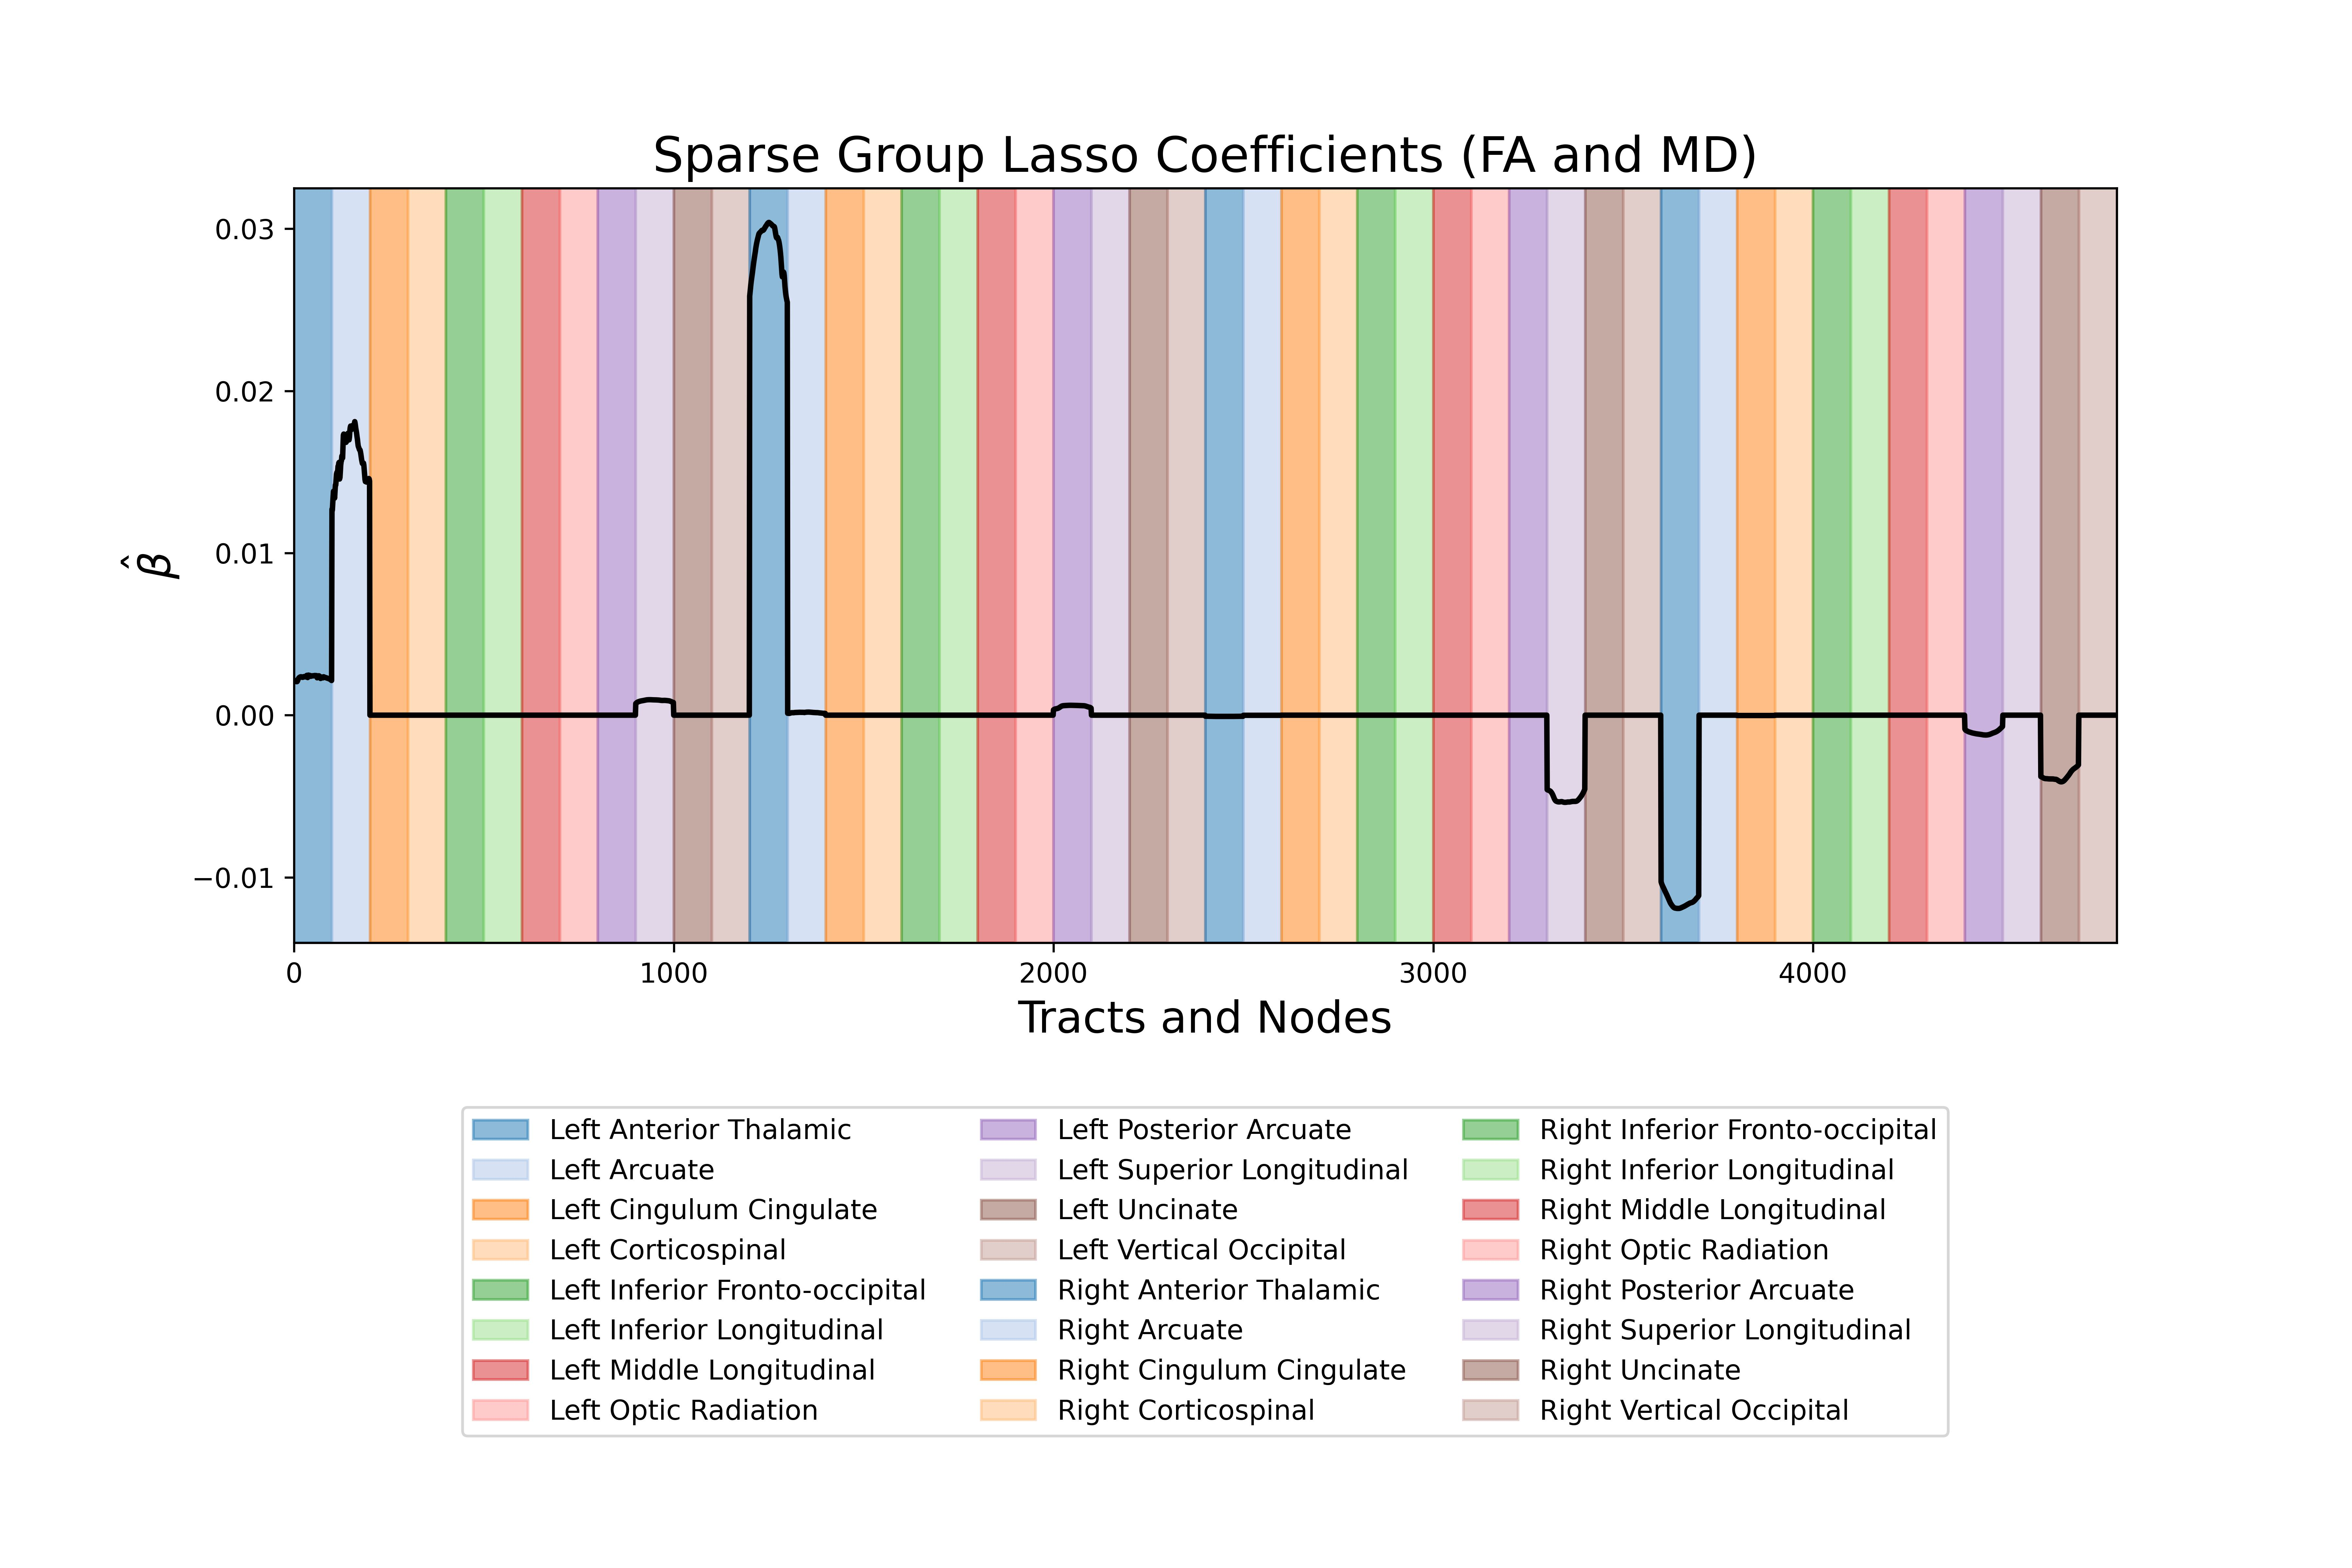
\includegraphics[trim=10 20 10 20,clip,width=0.8\textwidth]{sgl.jpg}
      \caption{Sparse Group Lasso with both phase encoding directions.}
    \end{figure}

    \begin{figure}
      \centering
      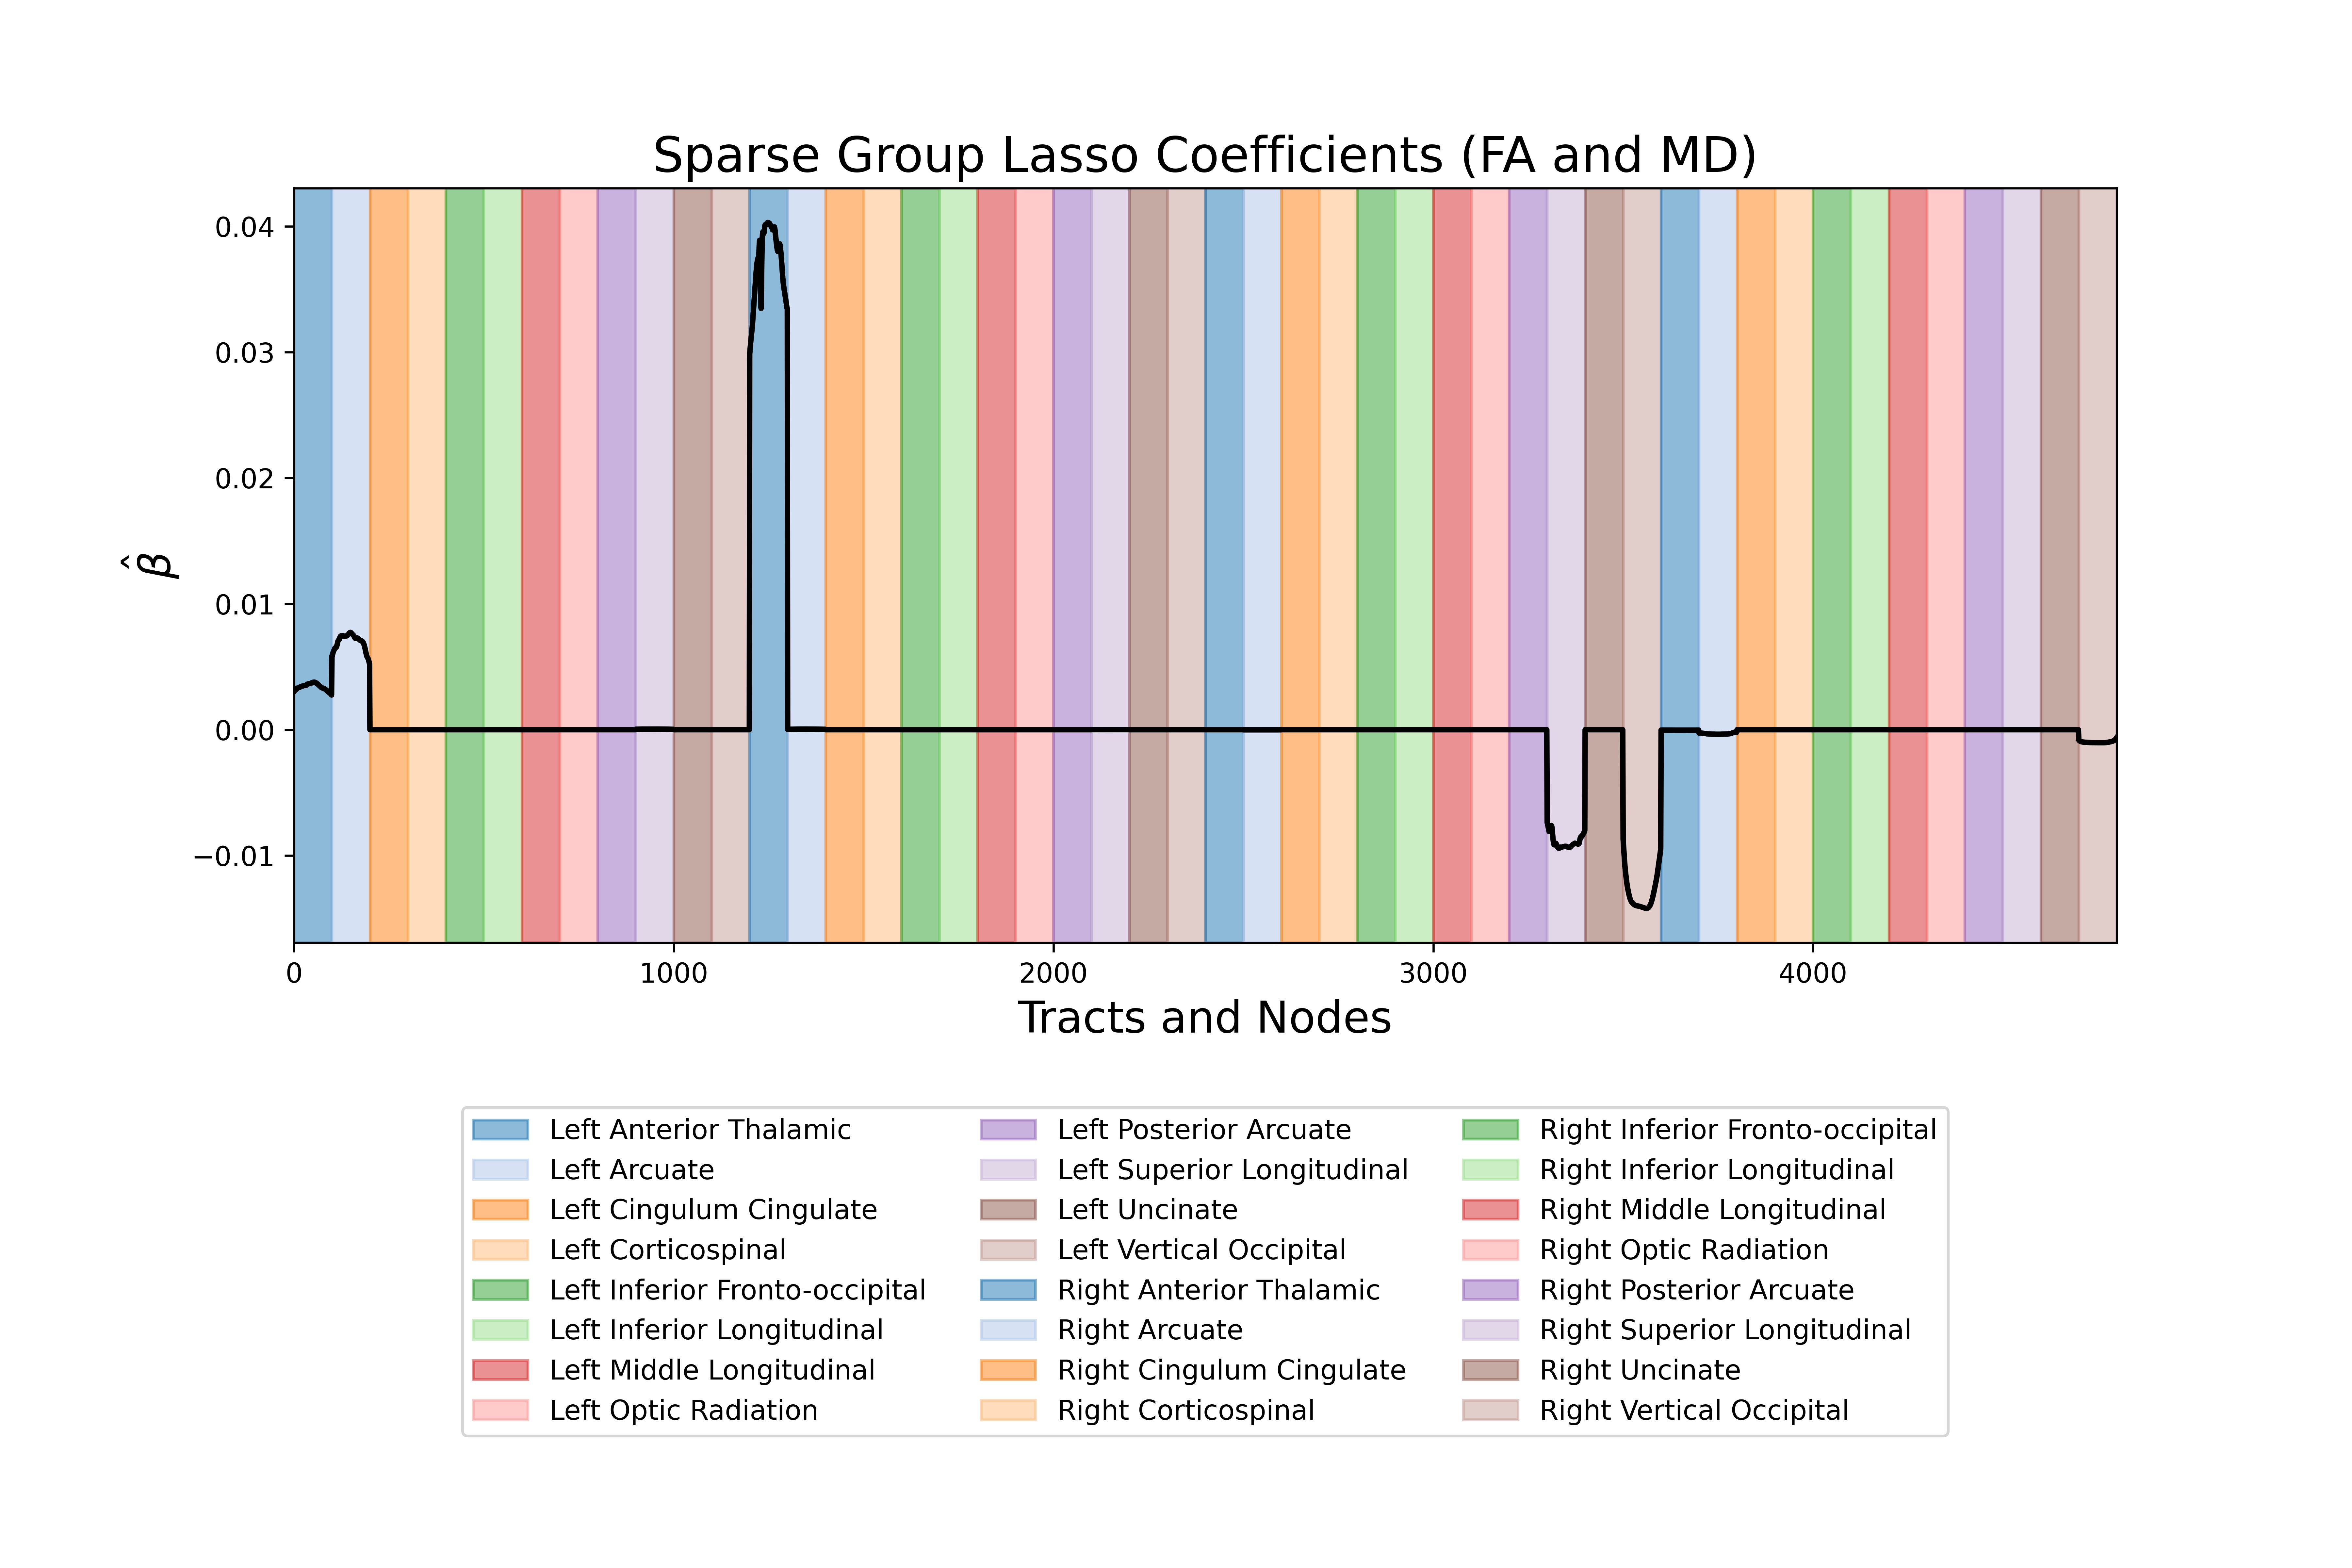
\includegraphics[trim=10 20 10 20,clip,width=0.8\textwidth]{sgl_nofmap.jpg}
      \caption{Sparse Group Lasso without reverse phase encoding direction.}
    \end{figure}

  \end{block}

\end{column}

\separatorcolumn

\begin{column}{\colwidth}

  \begin{block}{Discussion}

    Features of white matter (WM) microstructure predicted PMA at scan, with better prediction of CA than GA. This finding likely relates to the timeline of WM development, where the vulnerability of oligodendrocytes is maximal between PMA of 24 to 48 weeks. We replicate previous findings that weights are distributed throughout WM, indicating that many regions of WM change over time, even in the first months of life after preterm birth. 

    Advantages of this data-driven approach include being able to utilize clinical scans collected under variable conditions, a continuously-maintained open-source preprocessing pipeline, and maximizing the use of neuroimaging data available without the need for \textit{a priori} feature engineering. Future research will consider whether WM microstructure relates to clinical status and developmental care during hospitalization. An accurate brain-age model for the neonatal brain holds potential for tracking the effects of neonatal care and predicting neurodevelopmental outcomes.

  \end{block}

  \begin{block}{Nullam vel erat at velit convallis laoreet}

    Class aptent taciti sociosqu ad litora torquent per conubia nostra, per
    inceptos himenaeos. Phasellus libero enim, gravida sed erat sit amet,
    scelerisque congue diam. Fusce dapibus dui ut augue pulvinar iaculis.

    \begin{table}
      \centering
      \begin{tabular}{l r r c}
        \toprule
        \textbf{First column} & \textbf{Second column} & \textbf{Third column} & \textbf{Fourth} \\
        \midrule
        Foo & 13.37 & 384,394 & $\alpha$ \\
        Bar & 2.17 & 1,392 & $\beta$ \\
        Baz & 3.14 & 83,742 & $\delta$ \\
        Qux & 7.59 & 974 & $\gamma$ \\
        \bottomrule
      \end{tabular}
      \caption{A table caption.}
    \end{table}

  \end{block}

  \begin{block}{References}

    \nocite{*}
    \renewcommand{\bibfont}{\scriptsize} % Use \footnotesize, \small, \scriptsize, or \tiny as needed
    \printbibliography

  \end{block}


\end{column}

\separatorcolumn
\end{columns}
\end{frame}

\end{document}
